

\chapter{High Valence Vertices}\label{ch:high_valence}

High valence vertices are a mesh feature which cause significant degredation in
DAGMC ray tracing performance. The valence of a vertex in a mesh is defined as
the number of edges connected to that vertex. \textit{High} valence vertices are
defined as vertices connected to an unusually large number of edges. This
region, known as a high valence region, will typically take on a fan-like shape
as seen in Figure \ref{fig:hv_example}.  The geometric origins of high valence
regions are typically a planar surface intersected with some form of curved
boundary condition. 

\begin{figure}[H]
  \centering
  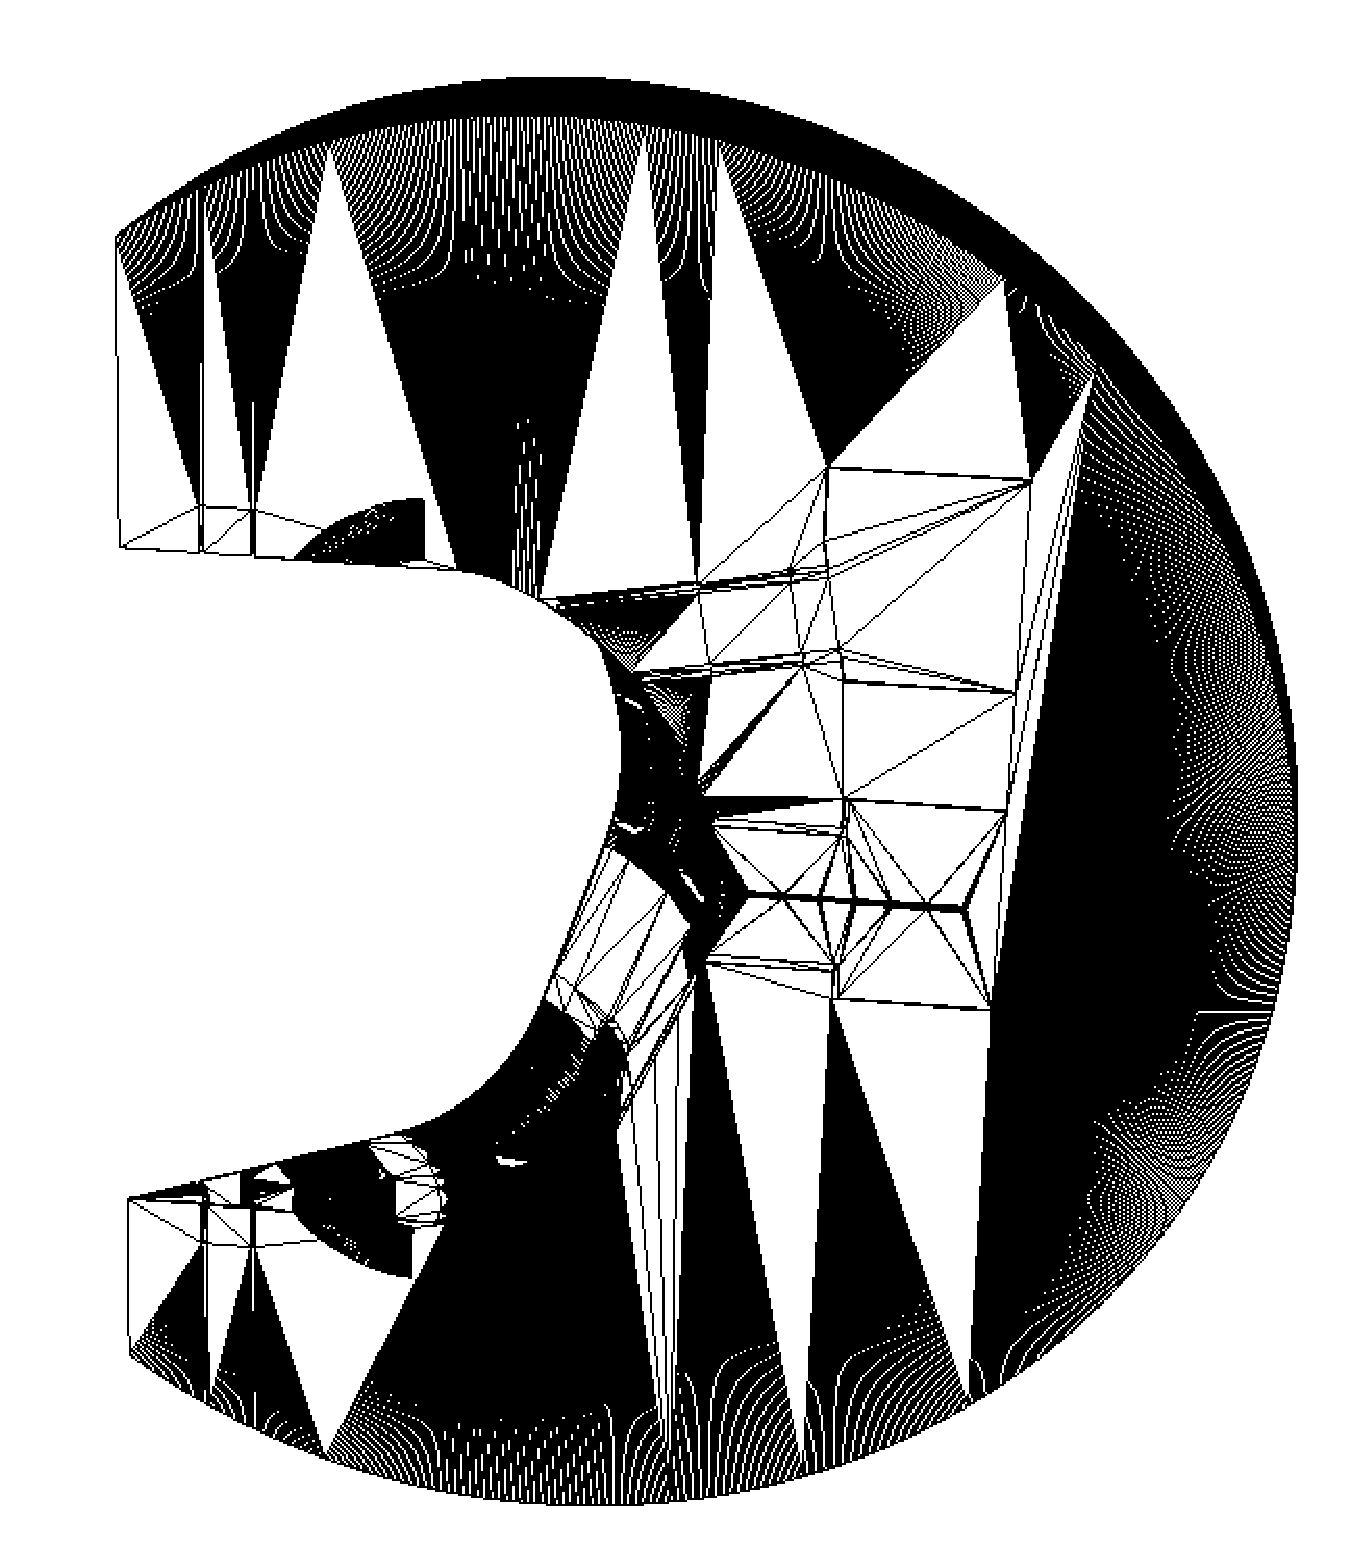
\includegraphics[scale=0.2]{iter_sideon.eps}
  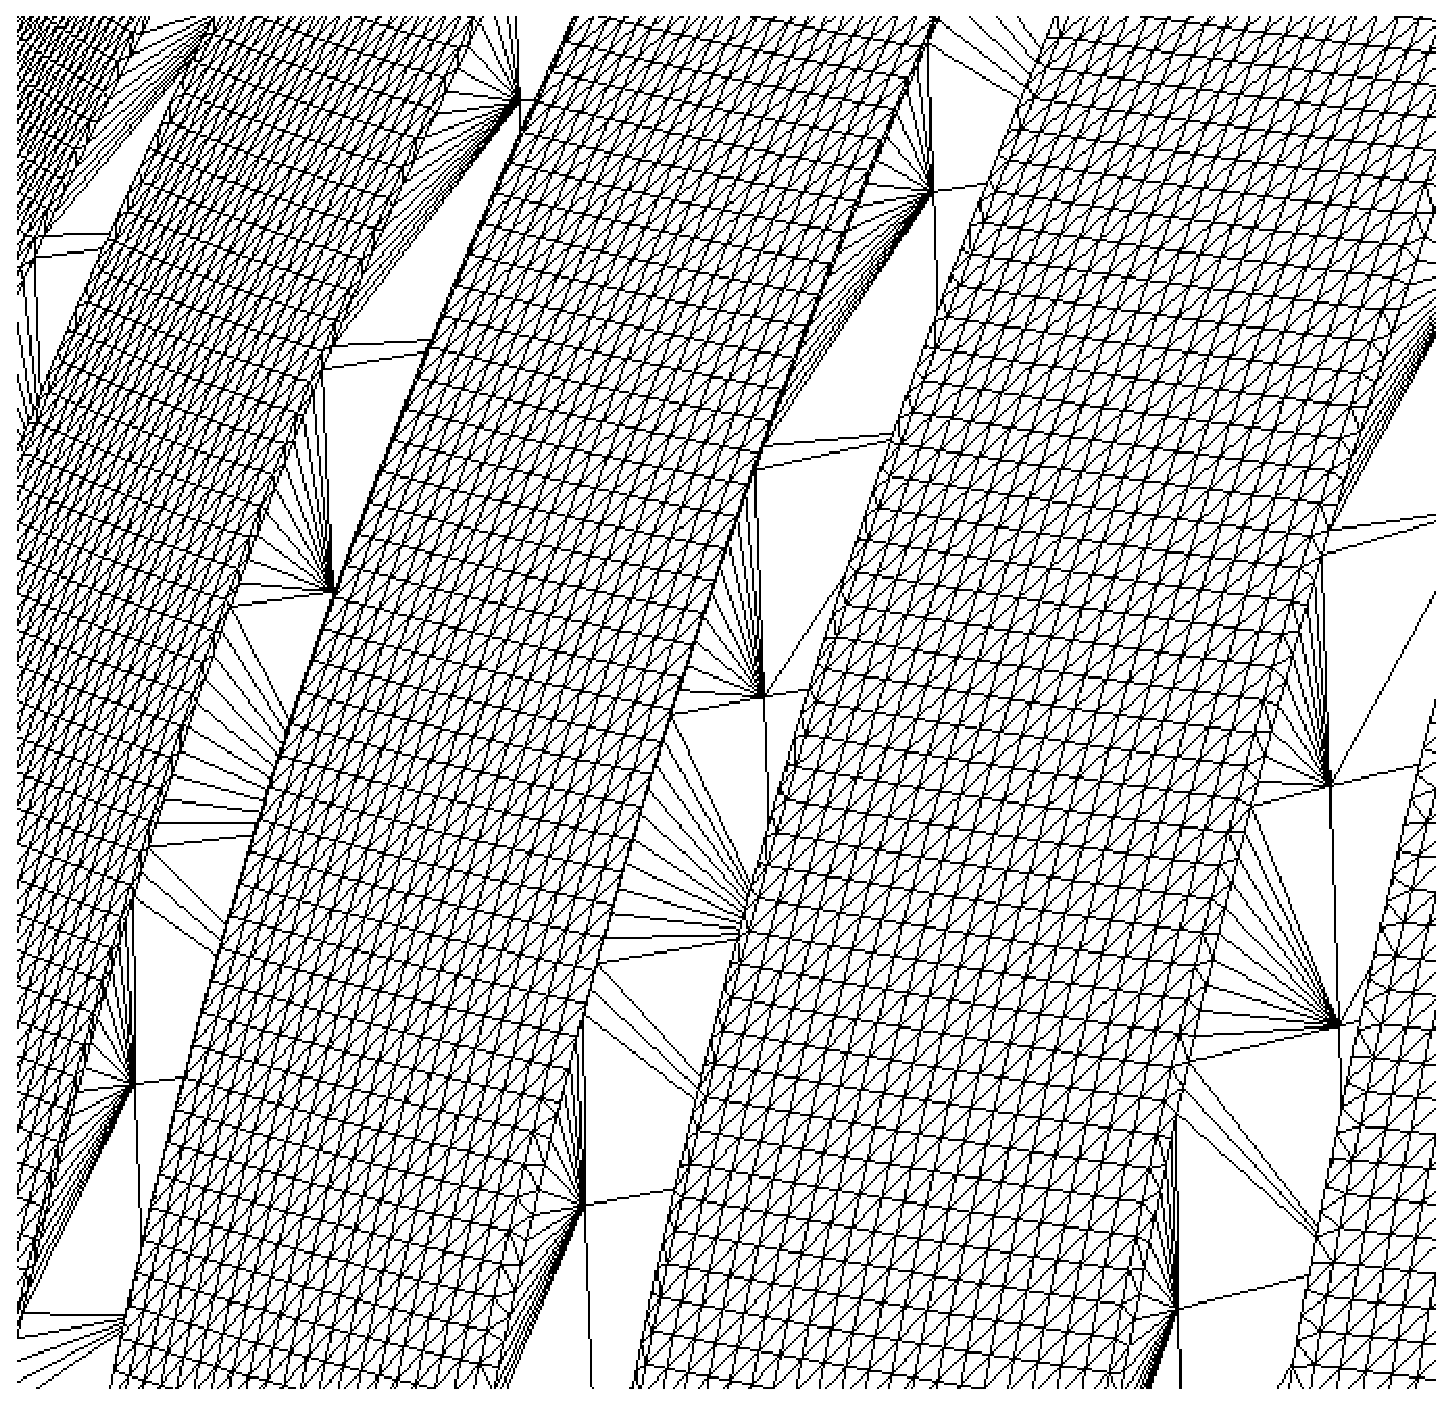
\includegraphics[scale=0.2]{ds_hv.eps}
  \caption{Examples of high valence vertices in analysis and test models.}
  \label{fig:hv_examples}
\end{figure}

These regions are commonly generated in the faceting algorithms used to produce
DAGMC meshes. This faceting scheme (which comes from ACIS libraries underlying
the CUBIT/Trelis graphics engine) is designed to produce the smallest number of
triangles possible to represent the model within the representation tolerance
specified in DAGMC's surface mesh generation preprocessing. This restriction is
favorable to the rasterization process commonly used to display models
interactively in the CAD program. Fewer triangles are better for the purpose
particle tracking in DAGMC as well as long as the geometry is accurately
represented. Even the ideal ray tracing acceleration structure queries for a
given triangle mesh scale as $O(log(N))$, and the size of models being analyzed
using the toolkit provides motivation to keep memory footprints as low as
possible. However, even with fewer triangles undesirable configurations can
impede performance as is shown by a set of tests conducted on models generated
by this faceting scheme.

A study conducted by Steve Jackson in 2010 on the performance of the MOAB ray
tracer revealed a steep degredation in performance with a decreasing faceting
tolerance or an increasing number of triangles. Using a DAGMC-based ray fire
test program, the performance of DAGMC's ray fire ability was evaluated for four
models. These models include a simple sphere, a notched or slotted sphere, and
an outer volume of an ITER model, shown in Figure \ref{fig:sj_hv_test_models}.

\begin{figure}[H]
    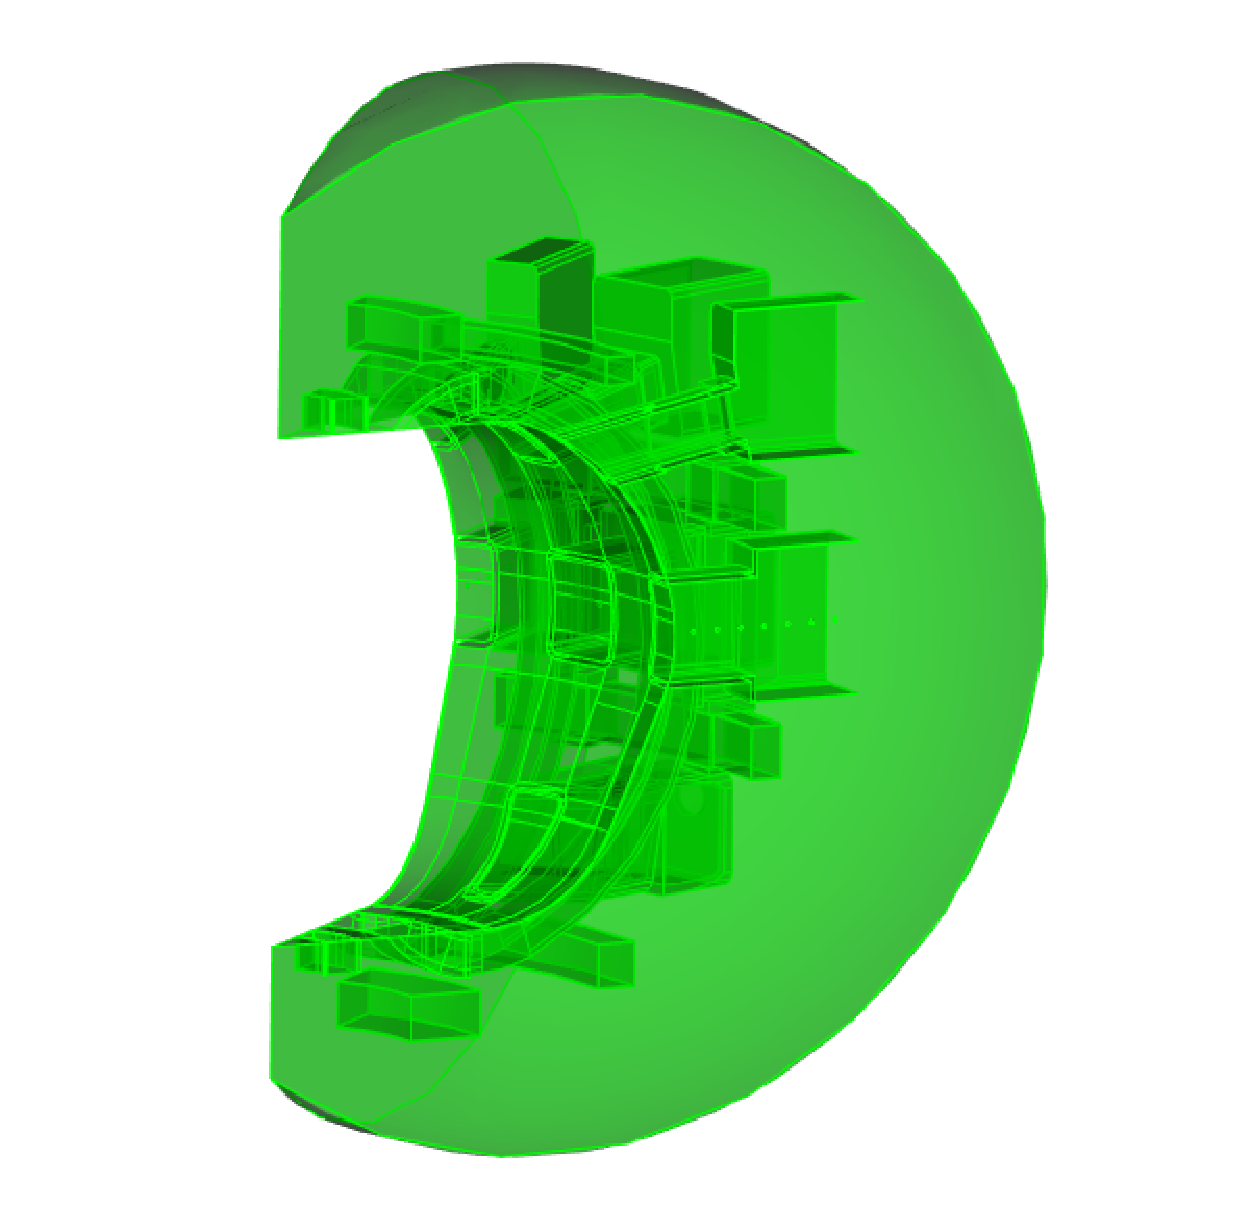
\includegraphics[scale=0.32]{iter_rf_vol.eps}
    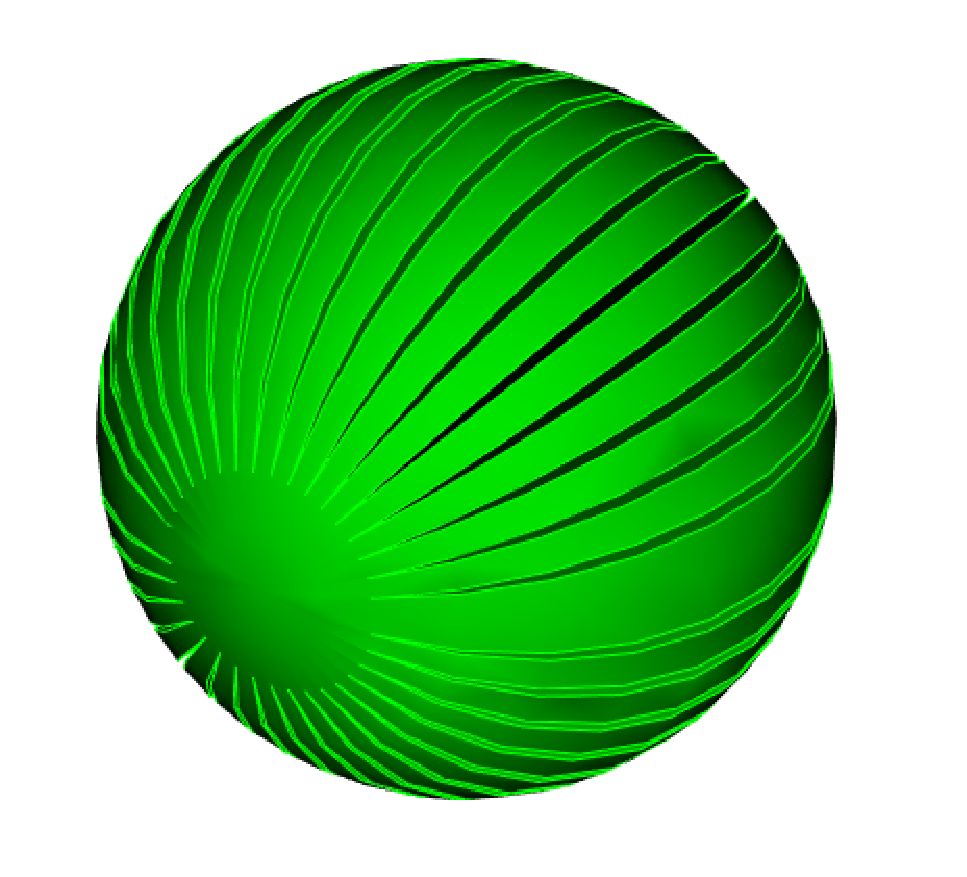
\includegraphics[scale=0.42]{ds.eps}
\begin{center}
  \caption{Images of the slotted sphere and ITER volume used to perform DAGMC
    ray fire performance tests with increasing number of triangles or,
    equivalently, decreasing faceting tolerance.}
\end{center}
\label{fig:sj_hv_test_models}
\end{figure} 

In each of these tests, the models are tesselated with an increasingly smaller
faceting tolerance where the faceting tolerance being defined as the maximum
distance between the faceted curve or surface and the geometric curve or surface
it resolves.  By this definition, the number of triangles needed to represent a
model is inversely proportional to the value of the faceting tolerance. An
increase in the number of triangles leads to a more complex nature of the
surface mesh in terms of BVH construction and traversal.

Each model used in these tests presents its own challenges with increasing
faceting tolerance. The sphere is a good control case for an increasing number
of triangles without change in complexity or exacerbation of pathological mesh
features. The number of triangles generated in the spherical case will tend
toward a maximum value with decreasing faceting tolerance, but the general
nature of the triangulated surface (triangle density, structure, etc.)  will
remain the same. This is not true of geometries with planar surfaces which may
be able to be resolved exactly using some finite number of triangles making the
sphere a vaulable test model in that regard. In the case of the notched sphere,
high-valence regions are generated by the faceting engine as a result of its
underlying algorithms for planar surfaces meeting curves surfaces. The high
triangle density of high valence regions causes overlaps in bounding volumes
which become larger as the faceting tolerance decreases. This results in
inefficient hierarchy traversal. Additionaly, and perhaps more importantly than
the presence of high valence regions, rays being fired with a point of origin at
the center of the model causes them to travel either exactly along or very near
to the surfaces of the planar slots in the sphere. Such a ray query will visit
many internal nodes of the hierarchy during traversal, creating what is referred
to as a very wide traversal through the BVH as opposed to a narrow traversal in
which fewer branches and fewer nodes of the tree are visited. In this way, the
slotted sphere provides a good measure for the performance of a wide traversal
through the hierarchy in a situation for which many of the internal nodes are
required to be visited. Finally, the faceting of a volume from an ITER model is
used as a production demonstration of the effect of high valence regions on
DAGMC performance (see Figure \ref{hv_examples}).

\begin{figure}[H]
  \begin{center}
    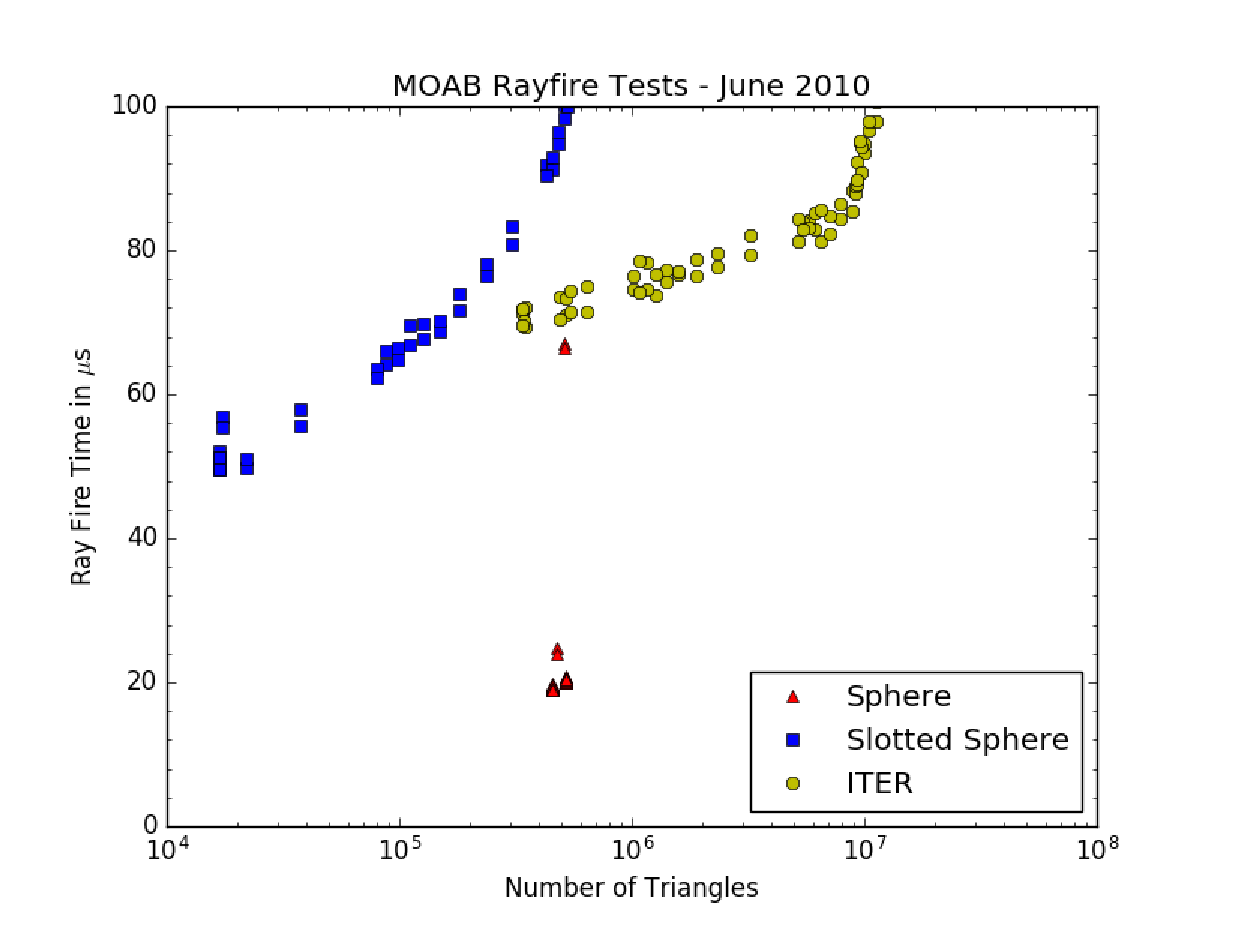
\includegraphics[scale=0.5]{sj_hv_test_results_2010.eps} \\
    \caption{Results of MOAB ray tracing performance tests with decreasing
      faceting tolerance performed by Steve Jackson in June of 2010. Data points
      represent average time spent in firing a ray for random rays
      originating at the center of each model.}
    \label{fig:sj_hv_test_results}
  \end{center}
\end{figure}

While the sphere model shows good scaling with increasing number of triangles,
the ITER volume and slotted sphere both have a pronounced increase in average
ray fire time with decreasing faceting tolerance. Knowing that both of the
latter models contain high valence regions, it was postulated at the time that
these regions had a significant effect on the scaling. In order to isolate the
high-valence vertex problem generated by the ACIS graphics faceting algorithm
used in Cubit/Trelis, a manually generated mesh was generated in MOAB with an
artificial high-valence region (shown in Figure \ref{hv_cube_design}). This mesh
is a modified cube centered on the origin in which the typical two-triangle
faceting has been replaced by a more complex planar surfce of triangles
including an interior high-valence region within the face. The high-valence
region was generated by inserting vertices along the diagonal of the interior
box and connecting them to the opposing corners of the box. This construction
was designed such that the valence of the corner vertices in the interior region
could be controled along with the size of the interior region relative to the
size of the entire face. Tests were then peformed by varing these two parameters
in order to characterize the performance impediment based on these two factors
and to determine its root cause.

\begin{figure}[H]
  \centering
    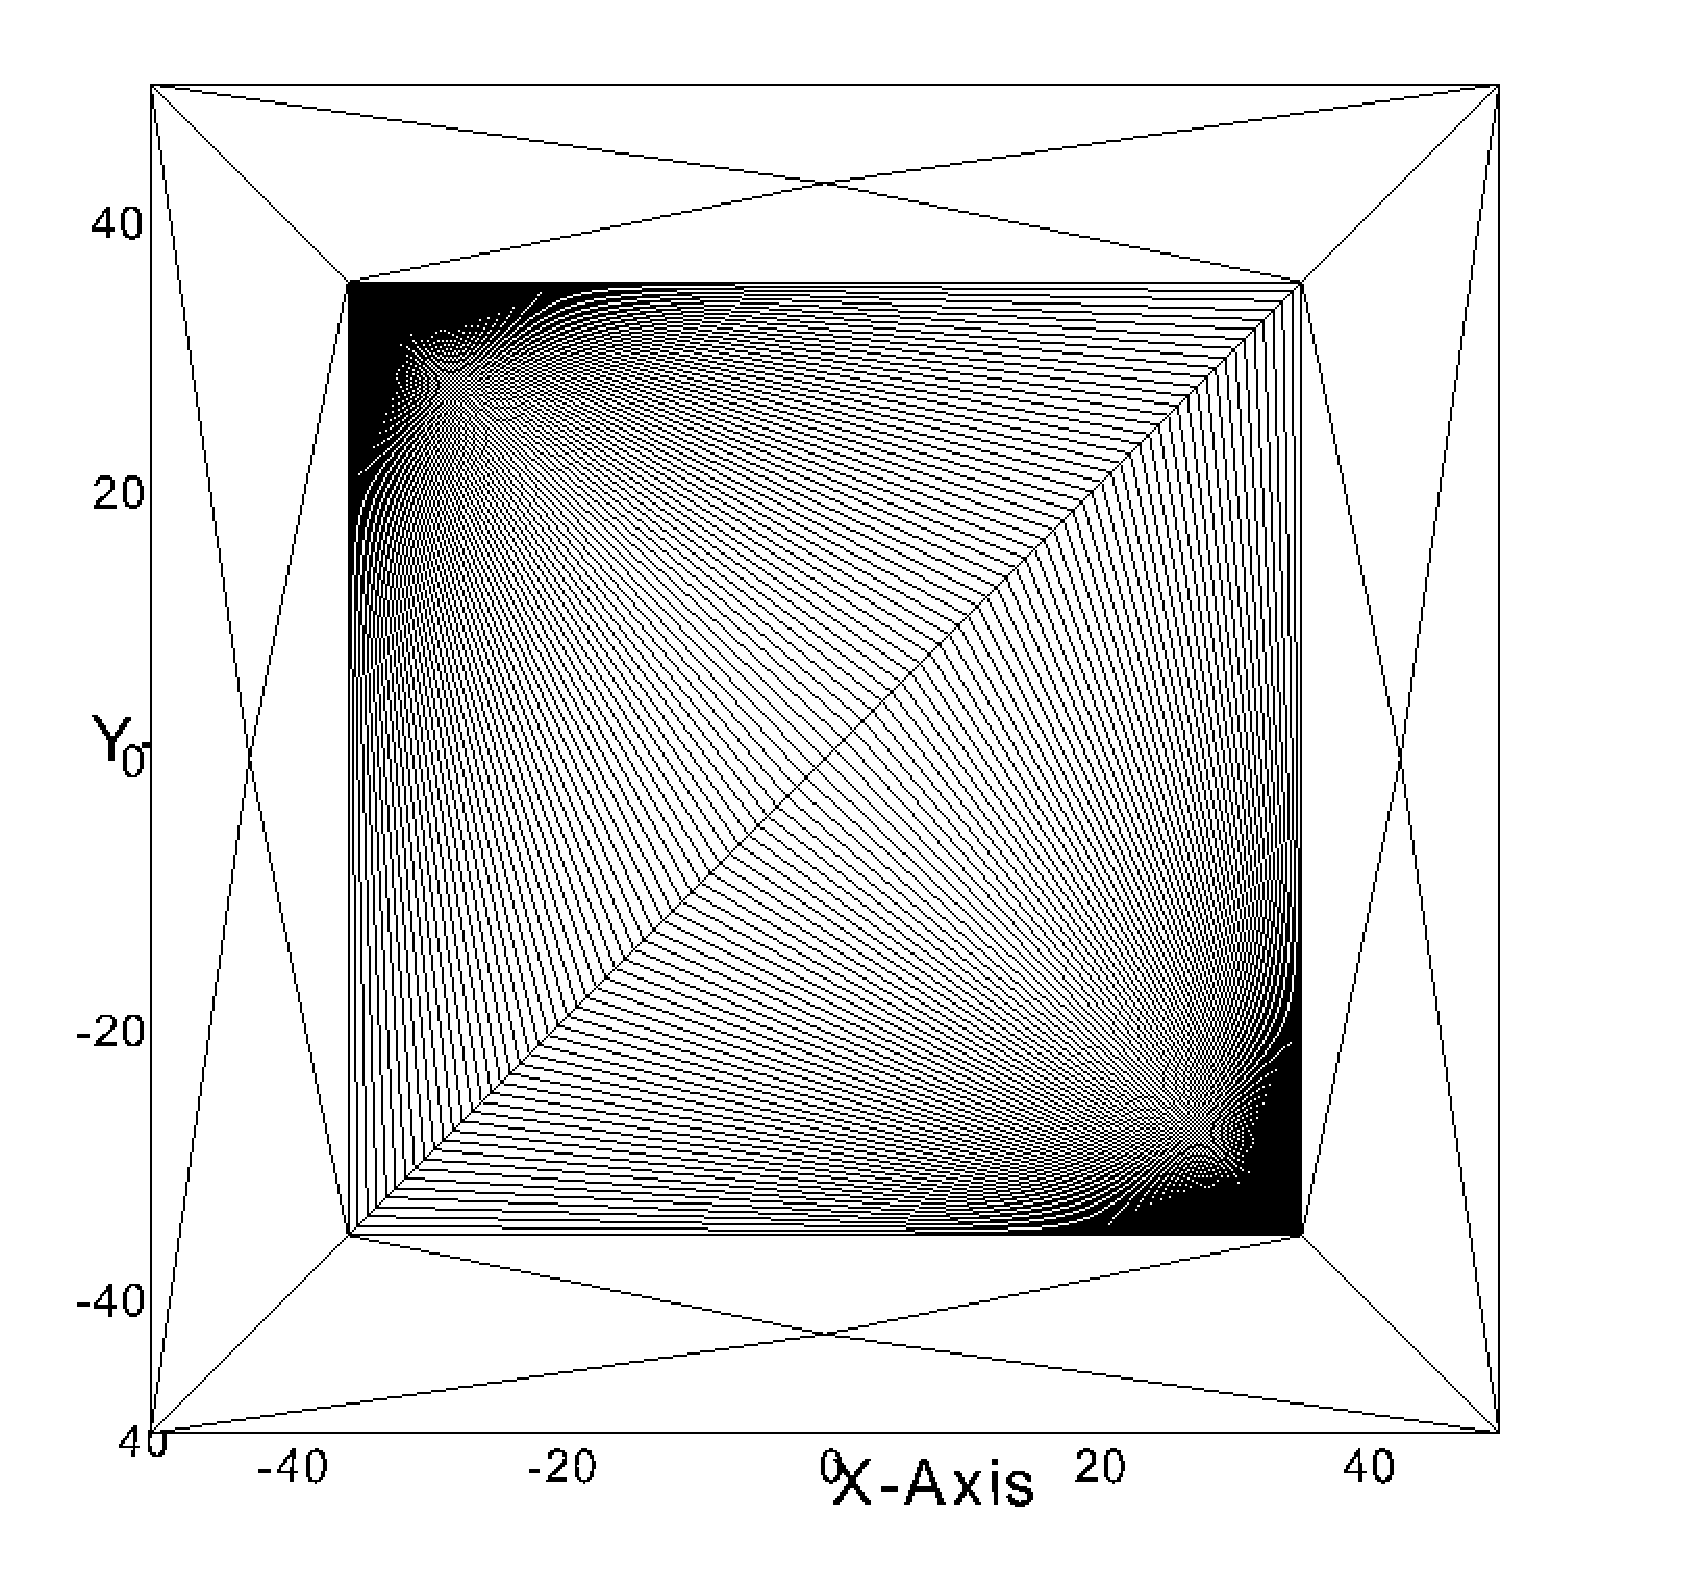
\includegraphics[scale=0.33]{hv_study_design.eps}
    \caption{Side-on view of the modified cube mesh used to study the high-valence vertex problem.}
    \label{hv_cube_design}
\end{figure}
